\section{Narzędzia programisty}

\begin{frame}[fragile]
  \frametitle{Narzędzia programisty}
  \framesubtitle{Wprowadzenie}

  Współczesne przeglądarki internetowe, posiadają wbudowane narzędzia, które pomagają w pracy programisty.

  \begin{itemize}
    \item inspektor drzewa DOM/stylów
    \item konsolę Web
    \item debugger
    \item podgląd \verb|local storage|, ciasteczek
    \item i inne
  \end{itemize}

  Dla nas, najciekawszym narzędziem będzie konsola.
\end{frame}


\begin{frame}[fragile]
  \frametitle{Narzędzia programisty}
  \framesubtitle{Wprowadzenie}

  Aby uruchomić narzędzia dla progamisty, należy w oknie przeglądarki wcisnąć przycisk \textbf{F12}.
\end{frame}


\begin{frame}[fragile]
  \frametitle{Narzędzia programisty}
  \framesubtitle{Firefox}

  \begin{figure}
    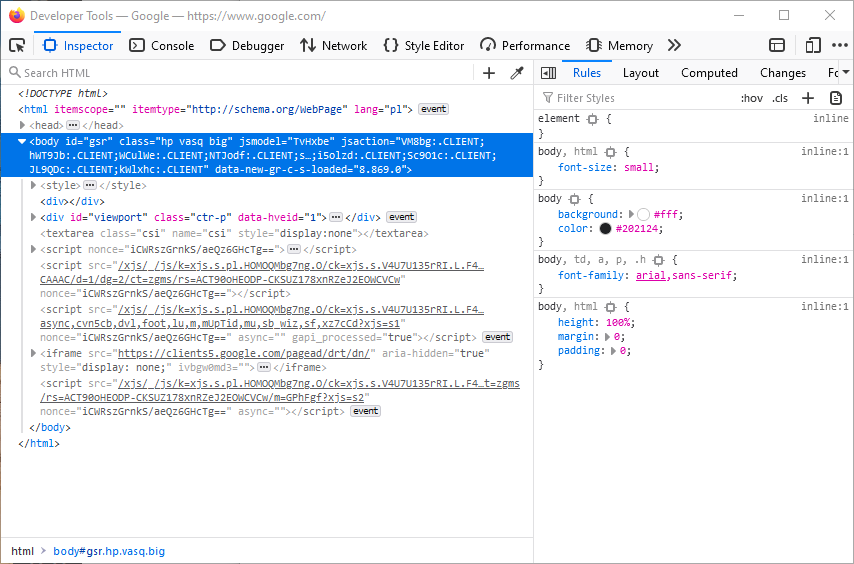
\includegraphics[scale=0.45]{images/dev-tools-firefox}
  \end{figure}

\end{frame}


\begin{frame}[fragile]
  \frametitle{Narzędzia programisty}
  \framesubtitle{Chrome}

  \begin{figure}
    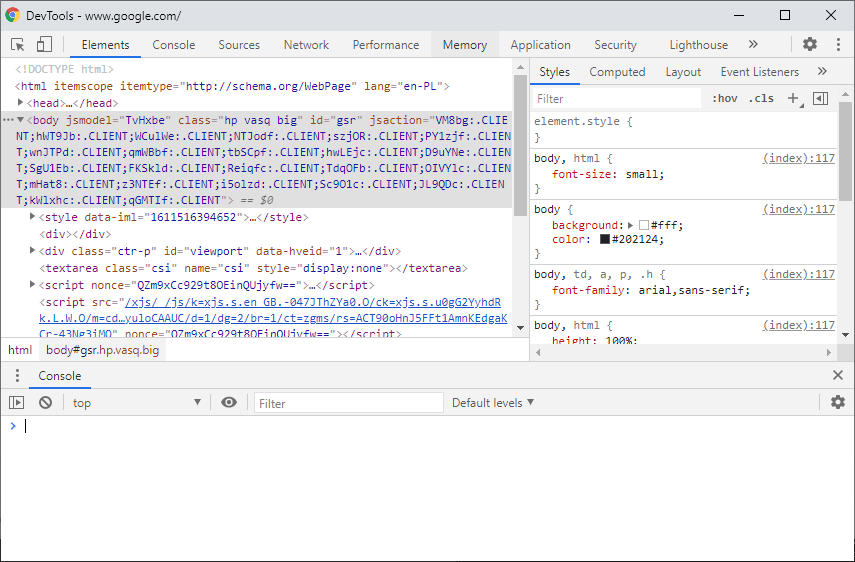
\includegraphics[scale=0.45]{images/dev-tools-chrome}
  \end{figure}
\end{frame}


\begin{frame}[fragile]
  \frametitle{Narzędzia programisty}
  \framesubtitle{Konsola}

  Konsola daje dostęp do interpretera języka \textbf{JavaScript}.

  \begin{itemize}
      \item podgląd błędów
      \item wywoływanie istniejącego kodu (funkcje)
      \item tworzenie zmiennych, funkcji
  \end{itemize}

  Jednak takie operacje nie są trwałe!
\end{frame}


\begin{frame}[fragile]
  \frametitle{Narzędzia programisty}
  \framesubtitle{Konsola}

  \begin{figure}
    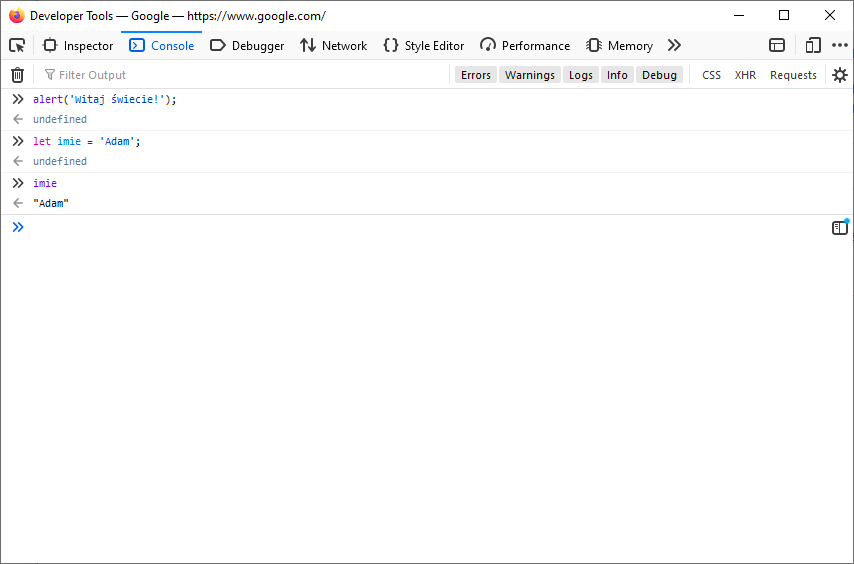
\includegraphics[scale=0.45]{images/dev-tools-console}
  \end{figure}
\end{frame}


\begin{frame}[fragile]
  \frametitle{Narzędzia programisty}
  \framesubtitle{Obiekt console}

  W trakcie tworzenia aplikacja, pojawia się potrzeba logwania róznych zdarzeń. Do tego celu służy obiekt \verb|console|.

  {\footnotesize
    \begin{itemize}
      \item \verb|console.log(obj1 [,obj2, ..., objN])| --- logowanie
      \item \verb|console.warn(obj1 [,obj2, ..., objN])| --- ostrzeżenie
      \item \verb|console.info(obj1 [,obj2, ..., objN])| --- informacja
      \item \verb|console.error(obj1 [,obj2, ..., objN])| --- błąd
    \end{itemize}
  }
\end{frame}


\begin{frame}[fragile]
  \frametitle{Narzędzia programisty}
  \framesubtitle{Obiekt console}

  Wszystkie metody działają bardzo podobnie. Wyświetlają przekazany argument w konsoli:

  \begin{minted}{js}
console.log('Ala ma kota');
console.info('Ala', 'ma', 'kota');
console.warn('Ala ma', 14, 'lat');
console.error('Kot ma Alę');
  \end{minted}

  \begin{figure}
    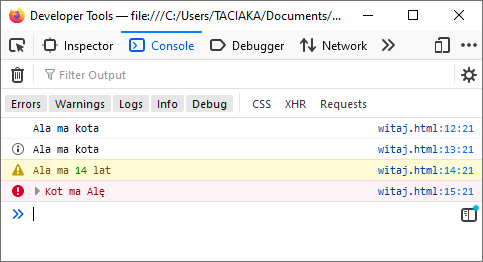
\includegraphics[scale=0.45]{images/dev-tools-console-example}
  \end{figure}


\end{frame}



